\documentclass{standalone}

\usepackage{tikz} % drawing in LaTeX

\begin{document}


    	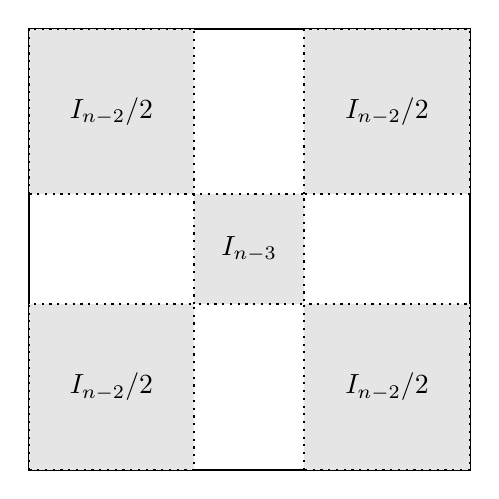
\begin{tikzpicture}[scale=.7]
    		\tikzstyle{blancEncadre}=[thick]
    		\tikzstyle{grisEncadre}=[thick, dotted, fill=gray!20]
    	
    		\draw [blancEncadre] (0,0) rectangle (8,8);
    		% molecular areas
    		\draw [grisEncadre] (0,0) rectangle (3,3) node [midway] {$I_{n-2}/2$};
    		\draw [grisEncadre] (0,5) rectangle (3,8) node [midway] {$I_{n-2}/2$};
    		\draw [grisEncadre] (5,0) rectangle (8,3) node [midway] {$I_{n-2}/2$};
    		\draw [grisEncadre] (5,5) rectangle (8,8) node [midway] {$I_{n-2}/2$};
    		% atomic area
    		\draw [grisEncadre] (3,3) rectangle (5,5) node [midway] {$I_{n-3}$};
    		
		\end{tikzpicture}

\end{document}